\subsection{Modelo de Gompertz}
El modelo de Gompertz, también llamado curva de Gompertz o función de Gompertz, es un modelo matemático para una serie temporal. La función es de tipo sigmoidea, y describe un crecimiento lengo en un periodo inicial y final, con uno más explosivo en un punto medio de la misma.

Inicialmente fue creada por Benjamin Gompertz para detallar su ley de la mortalidad humana, que se basa en un supuesto de que la resistencia de una persona a la muerte disminuye a medida que aumentan sus años, y fue descrito de la siguiente manera:

\begin{equation}
    N(t) = N(0) exp( -c ( exp(at) - 1))
\end{equation}

En esta ecuación, $N(t)$ representa un numero de individuos en un tiempo determinado $t$, por lo mismo, $N(0)$ representa la población inicial. $a$ denota una asíntota, $b$ y $c$ son valores positivos, que representan el desplazamiento a través del eje de las abcisas y la tasa de crecimiento, respectivamente. $exp$ denota la función exponencial.

\begin{figure*}
    \includegraphics[width=\textwidth]{casos diarios españa.png}
    \caption{Casos diarios de españa entre Marzo y Julio de 2020, fuente: cnecovid.isciii.es}
    \label{diarios españa}
\end{figure*}

En la publicación hecha por Sánchez-Villegas y colaboradores\cite{sanchez-villegas_codina_2020}, creada durante el año 2020, ellos decidieron utilizar el modelo de Gompertz para hacer una predicción del comportamiento de la epidemia de COVID-19 en España. Utilizando los datos de casos confirmados durante 47 días, generaron una curva de Gompertz que se ajustara lo más posible a sus datos.

¿Fue realmente acertado? Si bien, con la perspectiva inicial de dos años a futuro con respecto de esta publicación no lo parece para nada, contextualizando un poco a los datos que se tenían en ese momento podemos notar que la predicción fue, de hecho, relativamente acertada. En la figura \ref{diarios españa} podemos observar los casos diarios que se observan a lo largo del país entre las fechas de Marzo de 2020 hasta Julio del mismo año. La predicción inicial hecha por Sánchez-Villegas y colaboradores solo contemplaba datos hasta el 30 de abril de ese año, y contaba con solo 47 días de información, sin embargo, lograron demostrar que el pico de infección de españa llegó, efectivamente, en marzo de ese año, y que los contagios diarios iban extinguiendose.

Por desgracia, esta predicción cayó a mitades de Julio de 2020 y otras veces a futuro con la aparición de nuevas variantes y nuevos picos de infección en España y otros países del mundo. Aún así, el uso de este modelo predictivo en España y, según el autor, en la provincia de Hubei, donde ocurrió el primer caso de COVID, probó ser acertado para el corto plazo (Escala de Meses).

\begin{figure}
    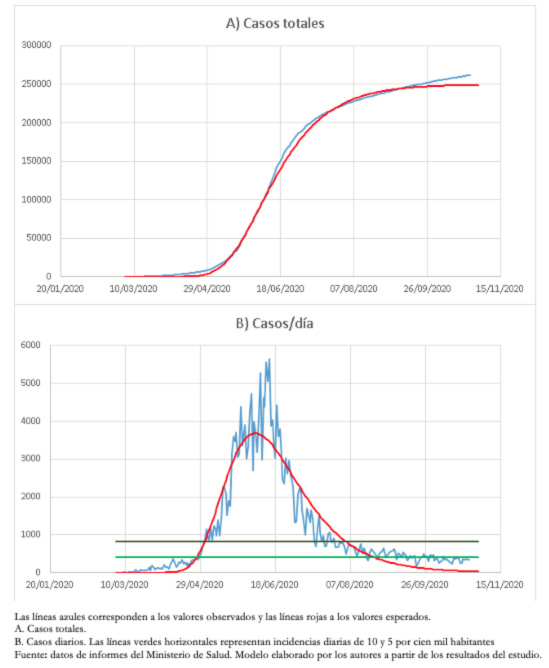
\includegraphics[width=\columnwidth]{gompertz en santiago.jpg}
    \caption{Modelo de Gompertz para Santiago. Fuente: \cite{canals_cuadrado_canals_2021}}
    \label{gompertz santiago}
\end{figure}

Para el caso de Santiago, el autor Canales y colaboradores\cite{canals_cuadrado_canals_2021}, han creado un modelo de Gompertz en el punto de claro aplanamiento de la curva de casos totales en la región, tal como muestra la figura \ref{gompertz santiago}. Este gráfico es relativamente tardío para poder hacer predicciones, sin embargo muestra como un modelo exitoso si podría haber dado resultados correctos si se hubiera encontrado antes.

Al mirar ambos gráficos se observa como se apegan ambos totalmente a lo esperado. El gran problema que se tiene entonces, es como llegar a este modelo cuando los datos que se tienen son insuficientes, y esta es la gran dicotomía que se encuentra cuando se trabaja con modelos de predicción: solo en retrospectiva se pueden validar.
